% --------------------------------------
% Document Class
% --------------------------------------
\documentclass[a4paper,11pt]{article}
% --------------------------------------



% --------------------------------------
% Use Package
% --------------------------------------


\usepackage[francais]{babel}
%\usepackage{ucs}
\usepackage[utf8]{inputenc}
\usepackage[T1]{fontenc}

\usepackage{makeidx}
\usepackage{color}
\usepackage{graphicx}
\usepackage{float}
\usepackage[hidelinks]{hyperref} 
\usepackage{geometry}
%\usepackage{lastpage}
%\usepackage{marginnote}
\usepackage{fancyhdr}
%\usepackage{titlesec}
%\usepackage{framed}
\usepackage{amsmath}
\usepackage{empheq}
\usepackage{array}
\usepackage{multicol}
\usepackage{csquotes}
%\usepackage{adjustbox}

% insert code
\usepackage{listings}

% define our color
\usepackage{xcolor}

% code color
\definecolor{ligthyellow}{RGB}{250,247,220}
\definecolor{darkblue}{RGB}{5,10,85}
\definecolor{ligthblue}{RGB}{1,147,128}
\definecolor{darkgreen}{RGB}{8,120,51}
\definecolor{darkred}{RGB}{160,0,0}

% other color
\definecolor{ivi}{RGB}{141,107,185}


\lstset{
    language=java,
    captionpos=b,
    extendedchars=true,
    frame=lines,
    numbers=left,
    numberstyle=\tiny,
    numbersep=5pt,
    keepspaces=true,
    breaklines=true,
    showspaces=false,
    showstringspaces=false,
    breakatwhitespace=false,
    stepnumber=1,
    showtabs=false,
    tabsize=3,
    basicstyle=\small\ttfamily,
    backgroundcolor=\color{ligthyellow},
    keywordstyle=\color{ligthblue},
    morekeywords={include, printf, uchar},
    identifierstyle=\color{darkblue},
    commentstyle=\color{darkgreen},
    stringstyle=\color{darkred},
}


% --------------------------------------



% --------------------------------------
% Page setting
% --------------------------------------
%\pagestyle{empty}
\setlength{\headheight}{15pt}

\setcounter{secnumdepth}{3}
\setcounter{tocdepth}{2}

\makeatletter
\@addtoreset{chapter}{part}
\makeatother 

\hypersetup{         % parametrage des hyperliens
  colorlinks=true,      % colorise les liens
  breaklinks=true,      % permet les retours à la ligne pour les liens trop longs
  urlcolor= blue,       % couleur des hyperliens
  linkcolor= black,     % couleur des liens internes aux documents (index, figures, tableaux, equations,...)
  citecolor= green      % couleur des liens vers les references bibliographiques
}

% --------------------------------------

% --------------------------------------
% Information
% --------------------------------------
\title{Compte-rendu TP9 TI : Détection de contours par approches du premier ordre}
\author{Elliot VANEGUE et Gaëtan DEFLANDRE}
% --------------------------------------

\definecolor{myColor}{rgb}{0.5, 0.1, 0.75}

% --------------------------------------
% Begin content
% --------------------------------------
\begin{document}

% Set language to english
  \selectlanguage{francais}

  % Start the page counting
  \pagenumbering{arabic}

  \maketitle
  
  \mbox{}
  \newpage
  \clearpage
  
  \section*{Introduction}
  Lors de ce TP, nous allons chercher à déterminer les contours d'une image grâce aux 
  gradients de ses pixels. Ces gradients portent de nombreuses informations qui peuvent
  être déterminé grâce à l'algorithme de Sobel, qui calcule le vecteur des gradients.
  
  \section{Seuillage de la norme d'un gradient}
  
  \subsection{Calcul de la norme d'un gradient par convolution}
  Nous avons dans un premier temps calculé les dérivées partielles de la fonction image dans les directions horizontales 
  et verticales. Pour cela, nous appliquons les filtres de Sobel
  $\begin{pmatrix}
     -1 & 0 & 1 \\
     -2 & 0 & 2 \\
     -1 & 0 & 1 
  \end{pmatrix}$ et 
   $\begin{pmatrix}
     -1 & -2 & -1 \\
     0 & 0 & 0 \\
     1 & 2 & 1
  \end{pmatrix}$
  afin de calculer le gradient de chaque pixel dans la direction x et y.
  Nous obtenons ainsi une image avec les contours dont la direction des pixels est horizontale et une seconde dont la direction est verticale.\\
  
  \begin{figure}[H]
  \center
   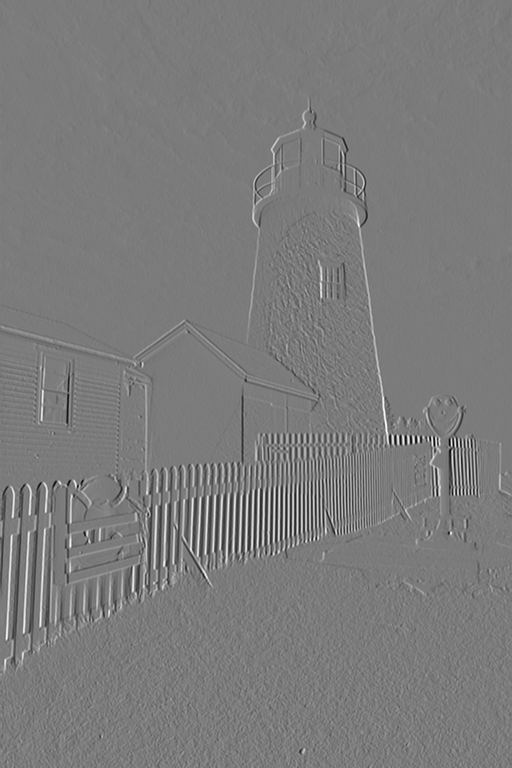
\includegraphics[width=4cm]{../lighthouse_8bits_grad_x.png}
   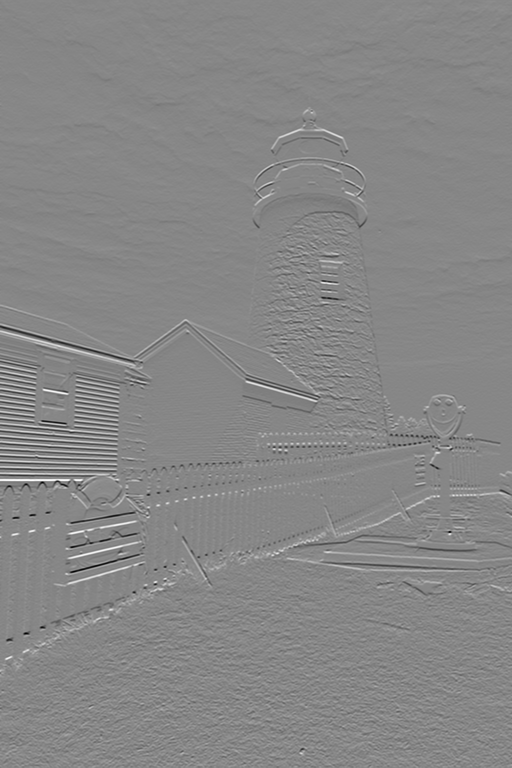
\includegraphics[width=4cm]{../lighthouse_8bits_grad_y.png}
   \caption{Images avec les contours horizontal et vertical}
  \end{figure}

  On voit sur ces deux images que les contours détectés par chaque filtre ne sont pas les mêmes
  à cause de leur direction. Grâce aux valeurs des pixels de ces deux images, nous calculons la norme
  des gradients dans une nouvelle image, ce qui fera ressortir les deux types de contours calculés précédemment
  sur celle-ci.

  \begin{figure}[H]
  \center
   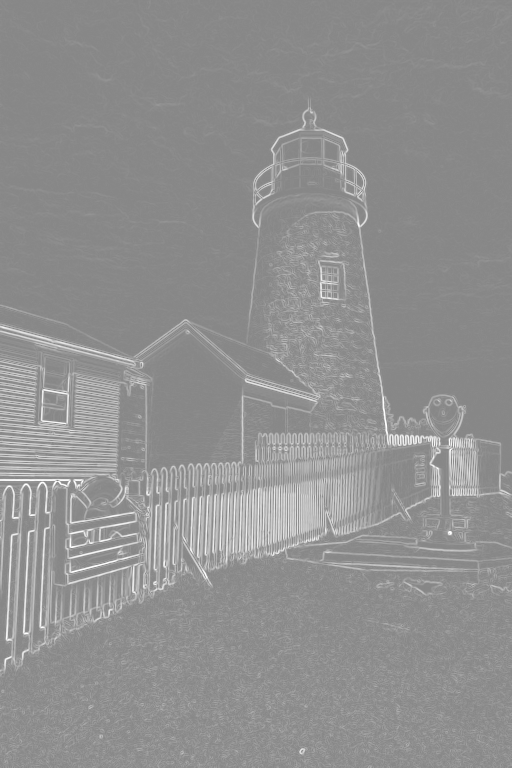
\includegraphics[width=4cm]{../norme32.png}
   \caption{Norme de l'image}
  \end{figure}
  
  On voit que la norme fait bien ressortir les contours, mais certains d'entre eux sont incomplets
  ou à l'inverse trop épais.\\

  Quand on regarde l'histogramme de l'image on voit que la valeur minimum des pixels est 0
  et le maximum est 904 pour l'image 32 bits. Pour calculer la norme de l'image nous utilisons
  la formule : $\sqrt{pX^2 + pY^2}$, ce qui explique la valeur assez importante du maximum. De plus
  l'image ne comporte pas de pixel noir, car les pixels gris foncé et noire sont dans les valeurs négatives
  que nous avons supprimées en faisant le carré de chaque pixel.\\

  Pour obtenir le même résultat que la fonction qui calcule la norme dans ImageJ, il faut passer
  l'image 32 bits en image 8 bits afin de passer d'un ensemble [-904;904] à un ensemble [0;255].\\
  
  \begin{figure}[H]
  \center
   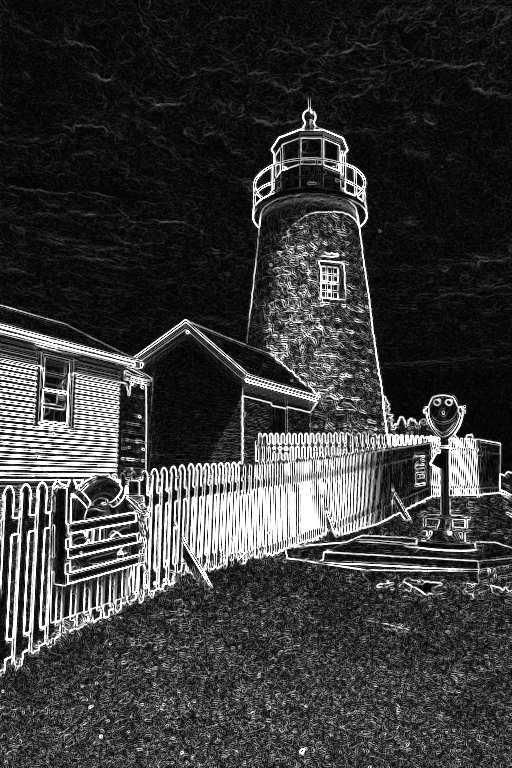
\includegraphics[width=4cm]{../norme8.png}
   \caption{Norme de l'image transformé en image 8 bits}
  \end{figure}
  
  Le résultat que nous obtenons est identique au résultat de la fonction d'ImageJ, car nous obtenons
  une image noire lorsque nous faisons la soustraction de notre résultat et celui d'ImgaJ.
  
  \subsection{Seuillage de la norme du gradient précédemment calculée}
  Grâce à l'outil ImgaeJ, nous seuillons l'image que nous avons calculée précédemment afin de la binariser.
  Nous utilisons dans un premier temps le seuillage automatique. On voit que le seuillage n'est pas très bon,
  car il y a encore beaucoup d'herbe visible dans l'image et il reste quelque pixel blanc dans l'image au niveau du ciel.\\
  
  \begin{figure}[H]
  \center
   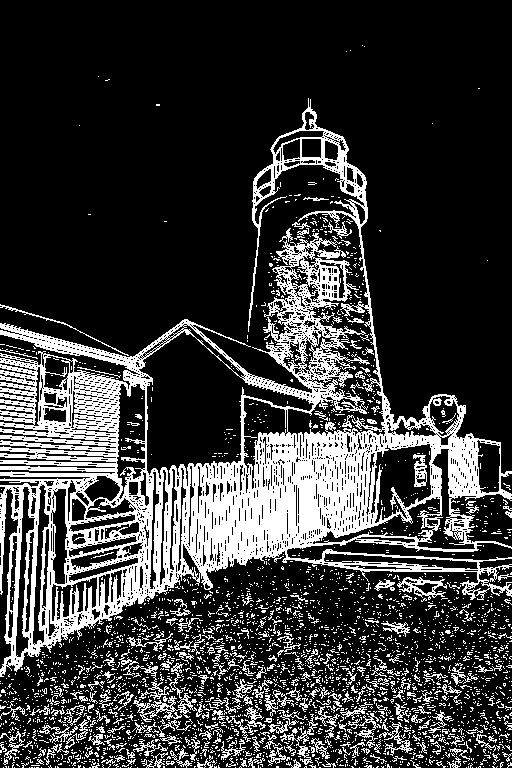
\includegraphics[width=4cm]{../binAuto.png}
   \caption{Binarisation automatique de l'image}
  \end{figure}
  
  Si nous diminuons ce seuil, le nombre de pixels blancs dans la pelouse et dans le ciel augmente. Et si
  nous augmentons le seuil, nous perdons certains contours du phare et de la maison. Finalement, nous déterminons que le seuil le plus 
  approprié doit se trouver entre 80 et 120.\\
  
  \begin{figure}[H]
  \center
   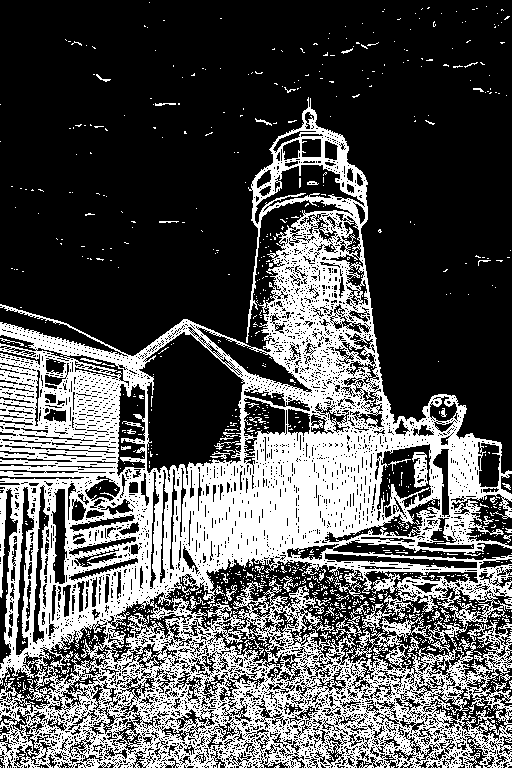
\includegraphics[width=4cm]{../bin50.png}
   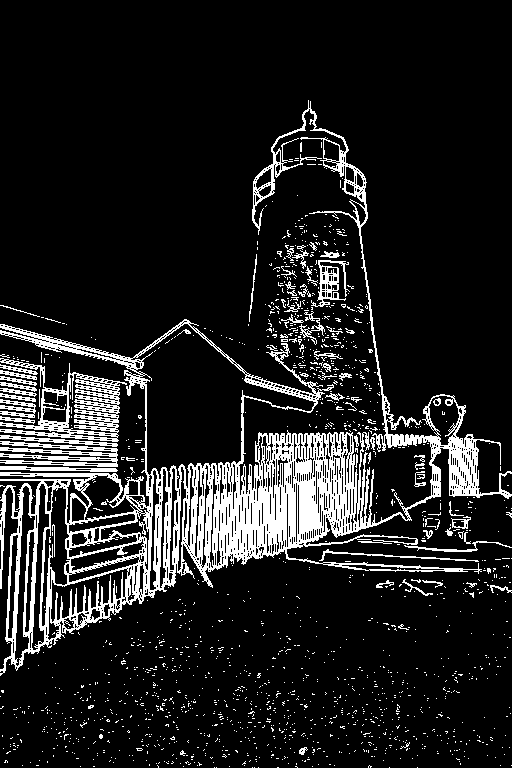
\includegraphics[width=4cm]{../bin140.png}
   \caption{Binarisation de l'image avec le seuil 50 puis 140}
  \end{figure}
  
  Afin d'affiner la détermination du seuil, nous calculons l'histogramme cumulé de l'image qui pour chaque valeur 
  de pixel ajoute la somme des valeurs des pixels précédents. A partir de cet histogramme, nous allons prendre comme 
  seuil le pixel à partir du quel l'histogramme commence à se stabiliser. Nous prenons donc le pixel qui est à peu près 
  à 20\% de l'histogramme, qui est le pixel 100.\\
  
  \begin{figure}[H]
  \center
   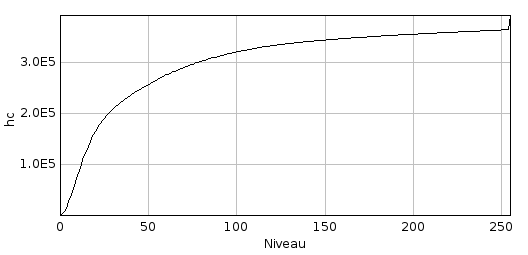
\includegraphics[width=10cm]{../histoCumul.png}
   \caption{Histogramme cumulé de l'image}
  \end{figure}
  
  \section{Détection des maxima locaux de la norme d'un gradient}
  Pour réaliser une détection des maxima locaux, nous avons besoin de calculer l'angle des gradients
  de l'image. Pour cela nous utilisons la formule suivante sur chacun des pixels :
  $$angle = atan2(pY, pX)/3.14*180$$
  
  Grâce à cet angle nous pouvons vérifier la valeur des deux pixels voisins qui le suive et si ces pixels
  voisins ont une valeur plus petite que le pixel traité, alors celui-ci appartient à un contour.
  Dans ce cas on passe les voisins à 0.\\
  
  \begin{figure}[H]
  \center
   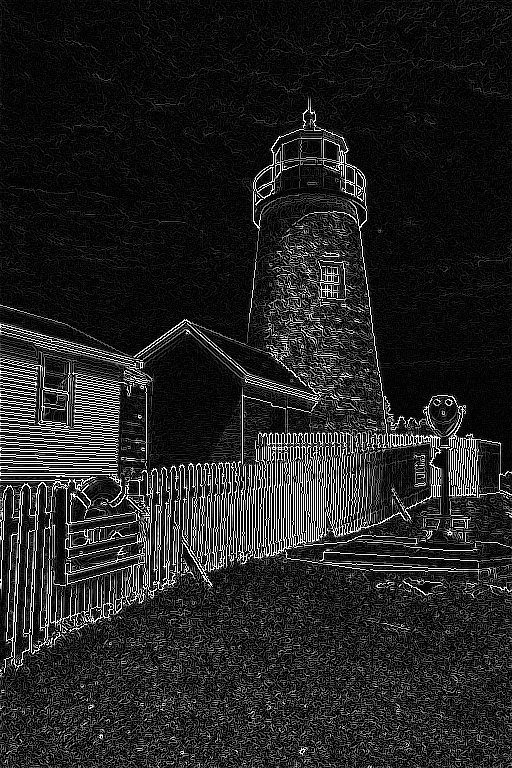
\includegraphics[width=7cm]{../maxima_locaux.png}
   \caption{Les maxima locaux de l'image}
  \end{figure}
  
  Nous pouvons voir qu'avec cette méthode les contours sont plus fins, ils ne sont composés que d'un pixel en largeur. 
  En revanche, cet algorithme ne supprime pas de bruit, il ne fait que diminuer la taille des contours.
  
  \section{Seuillage des maxima locaux par hystérésis}
  
  Maintenant que nous disposons des maxima locaux extrait à partir des normes et des gradients, nous 
  pouvons encore améliorer les résultats avec un seuillage par hystérésis. Ce seuillage consiste à prendre 
  deux seuil, avec un premier passage:
  \begin{itemize}
   \item pour le seuil haut: les maxima supérieurs à ce seuil sont considéré comme pixels contours.
   \item pour le seuil bas: les maxima inférieurs à ce seuil sont directement rejeté.
  \end{itemize}
  
%   Ensuite, pour les valeurs entre les deux seuils, un second passage est nécessaire. Pour chaque 
%   pixel situé rendre les deux seuils, si ces voisins sont au dessus du seuil haut alors ils sont eux aussi 
%   considéré comme contours sinon il est rejeté.\\
  Ensuite, pour les valeurs entre les deux seuils, un second passage est nécessaire. Pour chaque
  pixel situé au-dessus du seuil haut nous vérifions si l'un de ses voisins fait partie des pixels entre les deux seuilles.
  Si c'est le cas, le pixel trouvé fait partie lui aussi du contour et on passe sa valeur à 255. On répète cette opération
  jusqu'à ce qu'il n'y est plus de pixels dont la valeur est différente de 0 ou 255.\\

  Ce principe a été développé par J. F. Canny et est implémenté dans certaines bibliothèques de
  traitement d'images telles que OpenCV.\\

  Pour développer cette fonctionnalité, nous créons un plugin ImageJ en java. Pour cela, il faut
  implémenter l'interface \textit{PlugInFilter} de l'API ImageJ, puis nous manipulons ensuite nos
  images avec les objets propres à l'API d'ImageJ.\\
 
  \begin{lstlisting}[caption=Fonction qui va déterminer si les contours entre les deux seuils sont corrects]
private void propaRec(final ImageProcessor imNormeG,
                      ImageProcessor imContours, 
                      final int seuilBas, 
                      final int x,
                      final int y) {

  // récupération des dimension de l'image
  int width = imNormeG.getWidth();
  int height = imNormeG.getHeight();

  int[] dx8 = new int[] { -1, 0, 1, -1, 1, -1, 0, 1 };
  int[] dy8 = new int[] { -1, -1, -1, 0, 0, 1, 1, 1 };

  // parcours des voisins
  for (int k = 0; k < 8; k++) {
    int xk = x + dx8[k], yk = y + dy8[k];
    // si le voisin dépasse de l'image on le passe
    if (xk < 0 || xk >= width)
      continue;
    if (yk < 0 || yk >= height)
      continue;

    // tous les voisins qui sont entre les deux seuil
    // sont des contours donc on les met a 255
    if (imContours.get(xk, yk) == 128) {
      imContours.set(xk, yk, 255);
      propaRec(imNormeG, imContours, seuilBas, xk, yk);
    }
  }
}
  \end{lstlisting}
  
  Le code documenté du plugin est présent en annexe.\\

  Voici le résultat du plugin, en itératif, nous retrouvons une image binaire où les nuages ne sont 
  plus présents.\\
  
  \begin{figure}[H]
  \center
   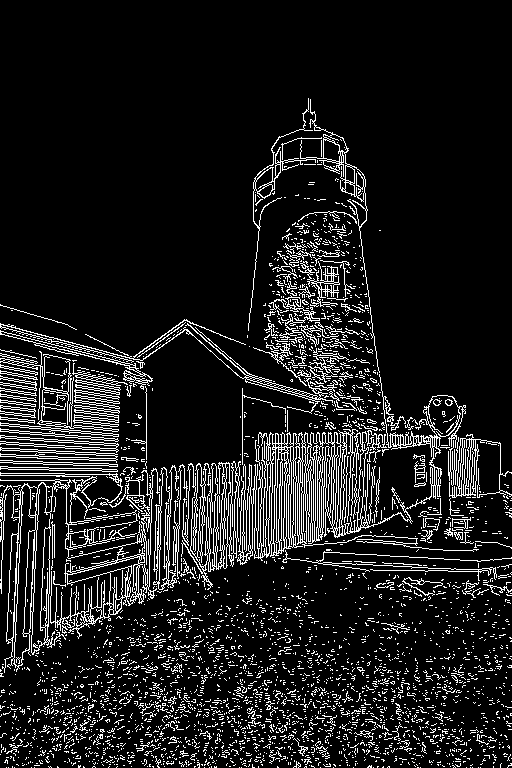
\includegraphics[width=7cm]{../canny_ite.png}
   \caption{Histogramme cumulé de l'image}
  \end{figure}
  
  \section{Conclusion}
  Les dérivées d'images sont efficaces pour la détections des contours, mais ces méthodes 
  extraient également beaucoup de bruit de l'image, qui n'est pas désirable. Pour diminuer ce bruit, des méthodes
  exsitent en utilisent la norme et le gradiants des pixels de l'image. Ensuite, différentes manières pour 
  binsariser les contours sont possibles, avec certaines statistiques tel l'histogramme cumulé ou en encore 
  le seuillage proposé par Canny, par hystérésis.
  
  
  \newpage
  
  \section{Annexe}
  
  \subsection{Les maxima locaux}
  
  \begin{lstlisting}[caption=Macro de calcul des maxima locaux]
/// Cette macro calcul pour une image:
/// - le gradient x
/// - le gradient y
/// - les normes
/// - les angles
/// - les maximas locaux
///
/// Elliot VANEGUE
/// Gaëtan DEFLANDRE
macro "norme_gradient" {

        // Calcul de la norme du gradient par masque de Sobel
        //
        requires("1.41i");      // requis par substring(string, index)
        setBatchMode(true);

        sourceImage = getImageID();
        filename = getTitle();
        extension = "";
        if (lastIndexOf(filename, ".") > 0) {
                extension = substring(filename, lastIndexOf(filename, "."));
                filename = substring(filename, 0, lastIndexOf(filename, "."));
        }
        filenameGradX = filename+"_grad_x"+extension;
        filenameGradY = filename+"_grad_y"+extension;

        gradX = sobelX(sourceImage,filenameGradX);
        gradY = sobelY(sourceImage,filenameGradY);
        
        /****** Calcul de la norme du gradient ******/
        // récupération de la taille de l'image
        W = getWidth();
        H = getHeight();
        
        run("Duplicate...", "title=norme");
        to32bits();
        imgNorme = getImageID();
        run("Duplicate...", "title=rounded_direction");
        to32bits();
        imgDirection = getImageID();
        
        // Calculs pour chaque pixel de la norme et de l'angle
        // avec arroundi de l'angle
        for(y=0; y<H; y++) {
                for(x=0; x<W; x++) {
                        norme = getNorme(x,y,gradX,gradY);
                        selectImage(imgNorme);
                        setPixel(x,y,norme);
                        angle = getAngle(x,y,gradX,gradY);
                        angle = roundAngle(angle);
                        selectImage(imgDirection);
                        setPixel(x,y,angle);
                }
        }
        
        selectImage(imgNorme);
        run("Duplicate...", "title=maxima_locaux");
        imgMaximaL = getImageID();

        //showaCruedHistogram();

        // Calculs des maxima locaux
        for(y=0; y<H; y++) {
                for(x=0; x<W; x++) {
                        selectImage(imgDirection);
                        angle = getPixel(x,y);
                        findMaxima(imgNorme, imgMaximaL, x, y, W, H, angle);
                }
        }
        selectImage(imgMaximaL);
        to8bits();

        setBatchMode("exit and display");
}


// ------------------------------------------------------------
// FONCTIONS
// ------------------------------------------------------------


/// Passe l'image courante en 32 bits
function to32bits(){
        //changement taille image pour éviter les nombres négatifs
        run("Conversions...", " ");
        run("32-bit");
}

/// Passe l'image courante en 8 bits
function to8bits(){
        run("Conversions...", " ");
        run("8-bit");
}

/// Calcul du gradient x de l'image 'imgSource' (filtre de sobel en x)
/// retourne l'image du gratient x en 32 bit, nommé 'filename' 
function sobelX(imgSource, filename) {
        selectImage(imgSource);
        run("Duplicate...", "title="+filename);
        to32bits();
        run("Convolve...", "text1=[-1 0 1\n-2 0 2\n-1 0 1\n] normalize");
        return getImageID();
}

/// Calcul du gradient y de l'image 'imgSource' (filtre de sobel en y)
/// retourne l'image du gratient y en 32 bit, nommé 'filename' 
function sobelY(imgSource, filename) {
        selectImage(imgSource);
        run("Duplicate...", "title="+filename);
        to32bits();
        run("Convolve...", "text1=[-1 -2 -1\n0 0 0\n1 2 1\n] normalize");
        return getImageID();
}

/// retourne l'angle exacte en degré, opération de trigo
/// en fonction du gradient x 'sobelx' et gradient y 'sobely'
function getAngle(x, y, sobelx, sobely){
        selectImage(sobelx);
        dx = getPixel(x, y);
        selectImage(sobely);
        dy = getPixel(x, y);
        theta = atan2(dy,dx);
        return (theta/3.1415)*180;
}

/// retourne la norme exacte, théorème de pythagore
/// en fonction du gradient x 'sobelx' et gradient y 'sobely'
function getNorme(x, y, sobelx, sobely){
        selectImage(sobelx);
        dx = getPixel(x, y);
        selectImage(sobely);
        dy = getPixel(x, y);
        return sqrt( dx*dx + dy*dy );
}

/// retourne l'arrondi de l'angle en paramètre au multiple de 45° le plus proche.
function roundAngle(angle){
        // premiere etage pour evite les virgule 
        // pour ne pas gérer les cas >= et <=
        angle = round(angle);

        // deuxieme etage on arroundit pour les 8 direction
        if (angle > -22.5 && angle < 22.5){
                return 0;
        } else if (angle > 22.5  && angle < 67.5){
                return 45;
        } else if (angle > 67.5  && angle < 112.5){
                return 90;
        } else if (angle > 112.5 && angle < 157.5){
                return 135;
        } else if (angle > 157.5 || angle < -157.5){
                return 180;
        } else if (angle < -22.5 && angle > -67.5){
                return -45;
        } else if (angle < -67.5 && angle > -112.5){
                return -90;
        } else if (angle < -112.5 && angle > -157.5){
                return -135;
        }
}

/// Cherche les maximas lacaux et fix les non maxima à 0. 
function findMaxima(imgNorme, imgMaximaL, x, y, W, H, angle){

        // cas compliqué à gérer
        if (x==0 || x>=W-1 || y==0 || y>=H-1){
                return;
        }
        
        selectImage(imgNorme);
        p = getPixel(x, y);

        if(angle == 0 || angle == 180){
                p1 = getPixel(x-1, y);
                p2 = getPixel(x+1, y);
                if (abs(p) >= abs(p1) && abs(p)>abs(p2)){
                        selectImage(imgMaximaL);
                        setPixel(x-1, y, 0);
                        setPixel(x+1, y, 0);
                }
        } else if (angle == 45 || angle == -135){
                p1 = getPixel(x-1, y-1);
                p2 = getPixel(x+1, y+1);
                if (abs(p) >= abs(p1) && abs(p)>abs(p2)){
                        selectImage(imgMaximaL);
                        setPixel(x-1, y-1, 0);
                        setPixel(x+1, y+1, 0);
                }
        } else if (angle == 90 || angle == -90){
                p1 = getPixel(x, y-1);
                p2 = getPixel(x, y+1);
                if (abs(p) >= abs(p1) && abs(p)>abs(p2)){
                        selectImage(imgMaximaL);
                        setPixel(x, y-1, 0);
                        setPixel(x, y+1, 0);
                }
        } else if (angle == 135 || angle == -45){
                p1 = getPixel(x-1, y+1);
                p2 = getPixel(x+1, y-1);
                if (abs(p) >= abs(p1) && abs(p)>abs(p2)){
                        selectImage(imgMaximaL);
                        setPixel(x-1, y+1, 0);
                        setPixel(x+1, y-1, 0);
                }
        }
}

/// Affiche l'histogramme cumulé de l'image courante
function showCruedHistogram(){
        // Histogramme cumulé
        getRawStatistics(surf, moy, min, max, std, h); // h[0..255] <-> histo
        hc=newArray(256);
        hc[0]=h[0];
        for (i=1;i< h.length;i++) {
                hc[i] = hc[i-1]+h[i] ;
        }
        Plot.create("Histogramme cumulé de "+getTitle, "Niveau", "hc", hc);
        Plot.show();
}
  \end{lstlisting}
  
  \newpage

  \subsection{Seuillage par hystérésis}
  
  \begin{lstlisting}[caption=Plugin pour le seuillage des maxima locaux par hystérésis]
import ij.ImagePlus;
import ij.plugin.filter.PlugInFilter;
import ij.process.ByteProcessor;
import ij.process.ImageProcessor;

import java.util.ArrayList;
import java.util.List;

public class _Contour implements PlugInFilter {

    private int seuilBas = 95;
    private int seuilHaut = 105;

    public int setup(String arg, ImagePlus imp) {
        return PlugInFilter.DOES_8G;
    }

    public void run(ImageProcessor ip) {
        ByteProcessor newbp = hystRec(ip, this.seuilBas, this.seuilHaut);
        ImagePlus newImg = new ImagePlus(
                                         "Résultat du seuillage par hystérésis", newbp);
        newImg.show();
    }

    public ByteProcessor hystIter(ImageProcessor imNormeG, int seuilBas,
                                  int seuilHaut) {

        // récupération des dimension de l'image
        int width = imNormeG.getWidth();
        int height = imNormeG.getHeight();

        // Création d'une image de la meme taille que l'image en entré
        ByteProcessor maxLoc = new ByteProcessor(width, height);
        List<int[]> highpixels = new ArrayList<int[]>();

        // parcours de l'image
        for (int y = 0; y < height; y++) {
            for (int x = 0; x < width; x++) {

                // on enleve les pixels en dessous du seuil bas
                int g = imNormeG.getPixel(x, y) & 0xFF;
                if (g < seuilBas)
                    continue;

                // si le pixel est supérieur au seuil haut
                // on ajoute le pixel à la nouvelle image et on met a jour la
                // liste
                // des pixels supérieurs au seuil haut
                if (g > seuilHaut) {
                    maxLoc.set(x, y, 255);
                    highpixels.add(new int[] { x, y });
                    continue;
                }

                // si le pixel est entre les deux seuil
                // on le met dans la nouvelle image
                maxLoc.set(x, y, 128);
            }
        }

        int[] dx8 = new int[] { -1, 0, 1, -1, 1, -1, 0, 1 };
        int[] dy8 = new int[] { -1, -1, -1, 0, 0, 1, 1, 1 };

        while (!highpixels.isEmpty()) {

            List<int[]> newhighpixels = new ArrayList<int[]>();

            for (int[] pixel : highpixels) {
                int x = pixel[0], y = pixel[1];

                // parcours des voisins
                for (int k = 0; k < 8; k++) {
                    int xk = x + dx8[k], yk = y + dy8[k];
                    // si le voisin dépasse de l'image on le passe
                    if (xk < 0 || xk >= width)
                        continue;
                    if (yk < 0 || yk >= height)
                        continue;

                    // tous les voisins qui sont entre les deux seuil
                    // sont des contours donc on les met a 255
                    if (maxLoc.get(xk, yk) == 128) {
                        maxLoc.set(xk, yk, 255);
                        newhighpixels.add(new int[] { xk, yk });
                    }
                }
            }

            highpixels = newhighpixels;
        }

        // tous les pixels qui n'ont pas été modifié ne sont
        // pas des contours donc on les met à 0
        for (int y = 0; y < height; y++) {
            for (int x = 0; x < width; x++) {
                if (maxLoc.get(x, y) != 255)
                    maxLoc.set(x, y, 0);
            }
        }
        return maxLoc;
    }

    public ByteProcessor hystRec(final ImageProcessor imNormeG,
                                 final int seuilBas, final int seuilHaut) {

        // récupération des dimension de l'image
        int width = imNormeG.getWidth();
        int height = imNormeG.getHeight();

        // Création d'une image de la meme taille que l'image en entré
        ByteProcessor maxLoc = new ByteProcessor(width, height);
        List<int[]> highpixels = new ArrayList<int[]>();

        // parcours de l'image
        for (int y = 0; y < height; y++) {
            for (int x = 0; x < width; x++) {

                // on enleve les pixels en dessous du seuil bas
                int g = imNormeG.getPixel(x, y) & 0xFF;
                if (g < seuilBas)
                    continue;

                // si le pixel est supérieur au seuil haut
                // on ajoute le pixel à la nouvelle image et on met a jour la
                // liste
                // des pixels supérieurs au seuil haut
                if (g > seuilHaut) {
                    maxLoc.set(x, y, 255);
                    highpixels.add(new int[] { x, y });
                    continue;
                }

                // si le pixel est entre les deux seuil
                // on le met dans la nouvelle image
                maxLoc.set(x, y, 128);
            }
        }

        propaRec(imNormeG, maxLoc, seuilBas, highpixels.get(0)[0],
                 highpixels.get(0)[1]);

        // tous les pixels qui n'ont pas été modifié ne sont
        // pas des contours donc on les met à 0
        for (int y = 0; y < height; y++) {
            for (int x = 0; x < width; x++) {
                if (maxLoc.get(x, y) != 255)
                    maxLoc.set(x, y, 0);
            }
        }
        return maxLoc;
    }

    private void propaRec(final ImageProcessor imNormeG,
                          ImageProcessor imContours, final int seuilBas, final int x,
                          final int y) {

        // récupération des dimension de l'image
        int width = imNormeG.getWidth();
        int height = imNormeG.getHeight();

        int[] dx8 = new int[] { -1, 0, 1, -1, 1, -1, 0, 1 };
        int[] dy8 = new int[] { -1, -1, -1, 0, 0, 1, 1, 1 };

        // parcours des voisins
        for (int k = 0; k < 8; k++) {
            int xk = x + dx8[k], yk = y + dy8[k];
            // si le voisin dépasse de l'image on le passe
            if (xk < 0 || xk >= width)
                continue;
            if (yk < 0 || yk >= height)
                continue;

            // tous les voisins qui sont entre les deux seuil
            // sont des contours donc on les met a 255
            if (imContours.get(xk, yk) == 128) {
                imContours.set(xk, yk, 255);
                propaRec(imNormeG, imContours, seuilBas, xk, yk);
            }
        }
    }
}

\end{lstlisting}

  
\end{document}  